\chapter{Design Phase}
\section{Object Oriented Analysis using UML}
\begin{wrapfigure}[5]{l}{4cm}

\includegraphics[width=4cm]{./images/implementation/uml}
\end{wrapfigure}
\paragraph{}The Unified Modeling Language (UML) is a standard language for specifying, visualizing, constructing, and documenting the artifacts
 of software systems, as well as for business modeling and other non-software systems. The UML represents
a collection of the best engineering practices that have proven successful in the modeling of large and complex systems. The UML is very important parts of developing
object oriented software and the software development process. The UML uses mostly graphical notations to express the design of software projects. Using the UML
helps projects teams communicate, explore potential designs, and validate the architectural design of the software.\par
\section{Use Case}
\paragraph{}We describes in this section, the general use case diagram so this use case describes the functionality provided by a system in terms
of actors, her we have two actors user(client) and admin, their goals represented as use cases, and any dependencies among those use case.
\begin{figure}[!h]
 \center
 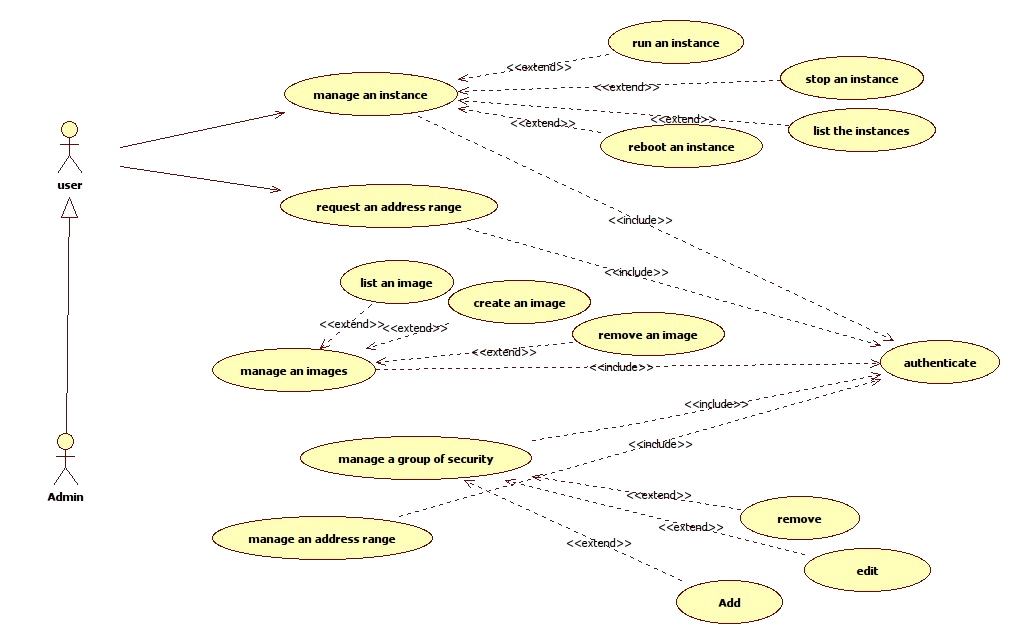
\includegraphics[width=16cm, height=12cm]{./images/design/usecase}
 \caption{Use Case Diagram}
\end{figure}

\section{Sequence diagram}
\paragraph{A sequence diagram}
\paragraph{}in a Unified Modeling Language (UML) is a kind of interaction diagram that shows how processes operate with one another and in what order. 
It is a construct of a Message Sequence Chart. A sequence diagram shows object interactions arranged in time sequence. 
It depicts the objects and classes involved in the scenario and the sequence of messages exchanged between the objects needed to carry out 
the functionality of the scenario. 
Sequence diagrams typically are associated with use case realizations in the Logical View of the system under development.\par
\paragraph{}Sequence diagrams are sometimes called event diagrams, event scenarios, and timing diagrams.\par

\begin{figure}[!h]
 \center
 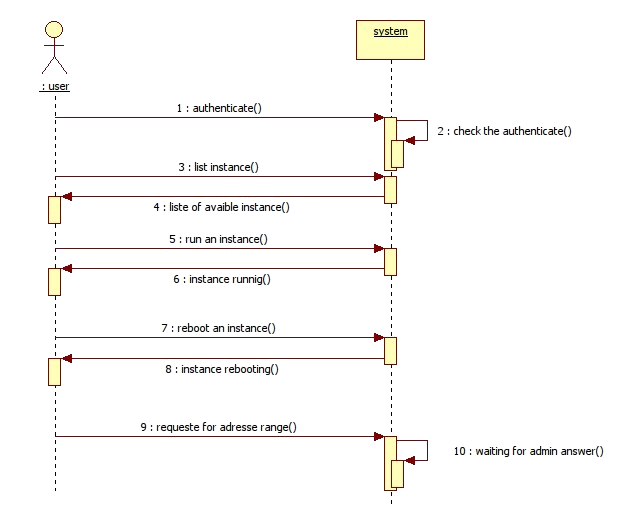
\includegraphics[width=18cm, height=15cm]{./images/design/sequenceuser}
 \caption{diagram sequance consumer}
\end{figure}

\begin{figure}[!h]
 \center
 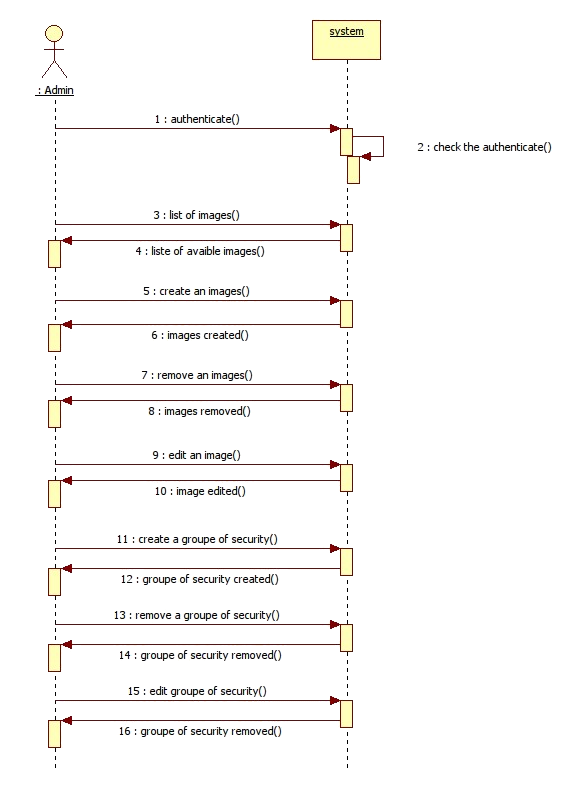
\includegraphics[width=16cm, height=19cm]{./images/design/sequenceadmin}
 \caption{diagram sequance admin}
\end{figure}

\clearpage

\section{Package Diagram}



\paragraph{}To move to the development, we rely on the principles of object-oriented approach. To this end, weare moving from a functional structure through the 
use case, to a structure object through the classes and packages. It is important to gather classes in packages to better understand the overall role of each
party and facilitate code maintenance. To identify the packages, we relied on two criteria: consistency and independence.

\begin{figure}[!h]
 \center
 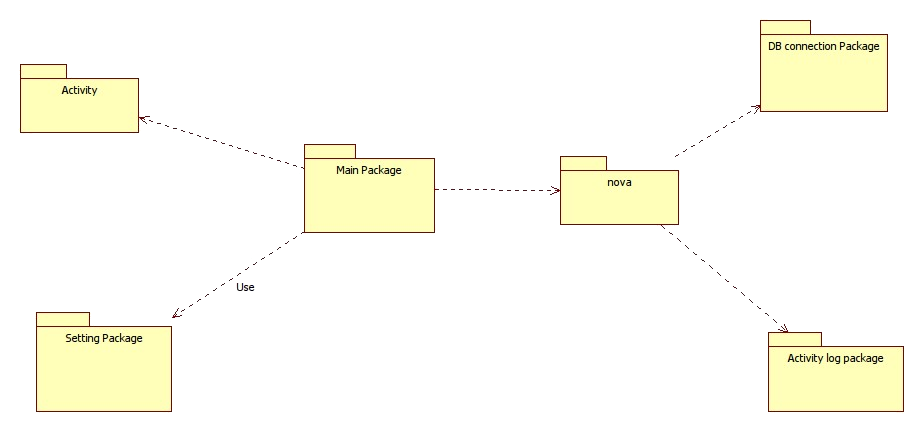
\includegraphics[width=12cm, height=10cm]{./images/design/package}
 \caption{diagram sequance admin}
\end{figure}
% \section{Class Diagram }
% \paragraph{}The class diagram is a static diagram. It represents the static view of an application.Class diagram
% is not only used for visualizing, describing and documenting different aspects of a system but also for constructing executable code of
% the software application. It describes the attributes and operations of a class and also the constraints imposed on the system, the class
% diagrams are widely used in the modeling of object oriented systems because they are the only UML diagrams which can be mapped directly with object oriented
% languages. The Class diagram pf our application is shown in the following figure.\par
\newpage
\section{Deployment Diagram}
\paragraph{}the deployment diagram shows the physical arrangement of materials that make up the distribution system and components of these materials.\par
\paragraph{}hardware resources are represented as nodes and these nodes are connected together by means of a communication medium.\par
\begin{figure}[!h]
 \center
 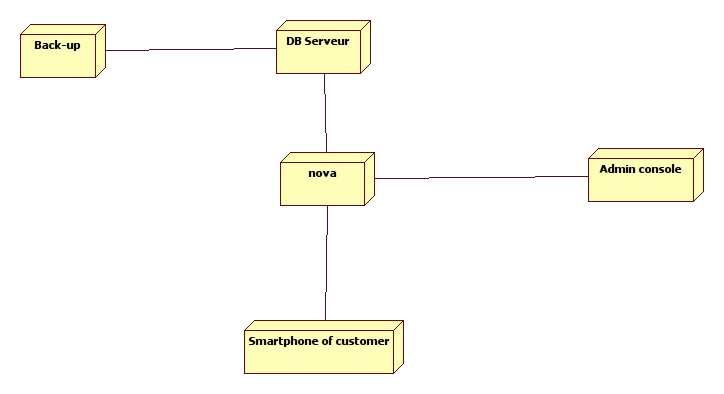
\includegraphics[width=12cm, height=8cm]{./images/design/deployment}
 \caption{Use Case Diagram}
\end{figure}

\section{Conclusion}
\paragraph{}
In the design phase the architecture was established, the different classes of the application are now classified, it is time for implementing our 
application